% =====================================================================
%  Native redraw of the pulse-profile geometry (after Poutanen &
%  Beloborodov 2006, MNRAS 373, 836, Fig. 1) in this paper's notation:
%  i (observer inclination), theta_s (spot colatitude), psi (spot-
%  observer angle), alpha (surface emission angle), varphi (phase).
%  Original drawing — no permission needed.
%
%  Build:  pdflatex geometry_figure.tex  ->  geometry_figure.pdf
% =====================================================================
\documentclass[border=8pt]{standalone}
\usepackage{amsmath}
\usepackage{tikz}
\usetikzlibrary{arrows.meta,calc}
\begin{document}
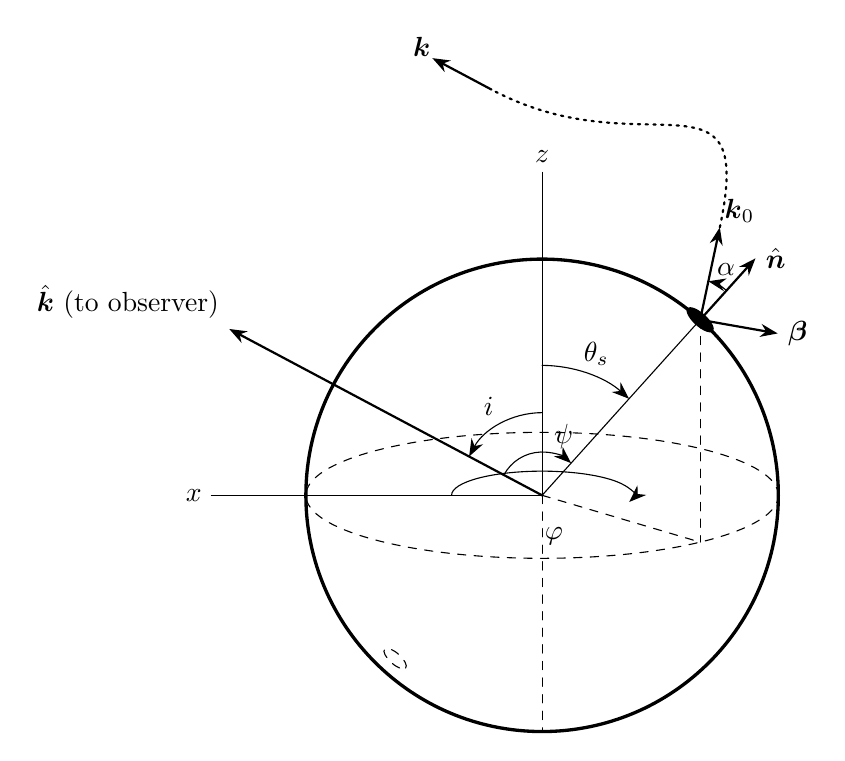
\begin{tikzpicture}[line cap=round, line join=round,
                    >={Stealth[length=2.2mm]}, scale=1.0]
  \def\R{3}
  \def\iang{62}      % inclination i, measured from +z toward the observer
  \def\thetas{42}    % spot colatitude theta_s, measured from +z
  \def\alphang{30}   % emission angle alpha, measured from the normal

  % ---- star, equator, axes -------------------------------------------
  \draw[very thick] (0,0) circle (\R);
  \draw[dashed] (0,0) ellipse ({\R} and 0.8);          % equatorial plane
  \draw[thin] (0,0) -- (0,{\R+1.1}) node[above] {$z$}; % spin axis
  \draw[dashed,thin] (0,0) -- (0,-\R);
  \draw[thin] (0,0) -- ({-\R-1.2},0) node[left] {$x$};

  % ---- observer direction, inclination i ------------------------------
  \draw[->,thick] (0,0) -- ({90+\iang}:{\R+1.5})
      node[above left] {$\hat{\boldsymbol{k}}$\ (to observer)};
  \draw[->] (0,1.05) arc[start angle=90, end angle={90+\iang}, radius=1.05];
  \node at ({90+\iang/2}:1.32) {$i$};

  % ---- spot at colatitude theta_s -------------------------------------
  \coordinate (S) at ({90-\thetas}:\R);
  \draw[thin] (0,0) -- (S);
  \fill[rotate around={-\thetas:(S)}] (S) ellipse (0.22 and 0.085);
  \draw[->] (0,1.65) arc[start angle=90, end angle={90-\thetas}, radius=1.65];
  \node at ({90-\thetas/2}:1.92) {$\theta_s$};

  % ---- spot--observer angle psi (between k-hat and the spot radius) ---
  \draw[->] ({90+\iang}:0.55) arc[start angle={90+\iang},
                                  end angle={90-\thetas}, radius=0.55];
  \node at (70:0.8) {$\psi$};

  % ---- surface normal and emission direction, angle alpha -------------
  \draw[->,thick] (S) -- ({90-\thetas}:{\R+1.05})
      node[right] {$\hat{\boldsymbol{n}}$};
  \draw[->,thick] (S) -- ++({90-\thetas+\alphang}:1.2)
      node[above right=-2pt] {$\boldsymbol{k}_0$};
  \draw[->] ($(S)+({90-\thetas}:0.5)$)
      arc[start angle={90-\thetas}, end angle={90-\thetas+\alphang}, radius=0.5];
  \node at ($(S)+({90-\thetas+\alphang/2}:0.72)$) {$\alpha$};

  % ---- spot velocity (azimuthal) ---------------------------------------
  \draw[->,thick] (S) -- ++(-10:1.0) node[right] {$\boldsymbol{\beta}$};

  % ---- bent photon trajectory: leaves along k0, arrives along k-hat ----
  \coordinate (P0) at ($(S)+({90-\thetas+\alphang}:1.2)$);
  \coordinate (Kend) at ($(P0)+(-2.9,1.75)$);
  \draw[dotted, thick]
      (P0) .. controls ($(P0)+({90-\thetas+\alphang}:2.2)$)
               and ($(Kend)+({\iang-90}:2.2)$) .. (Kend);
  \draw[->,thick] (Kend) -- ++({90+\iang}:0.85)
      node[above left=-3pt] {$\boldsymbol{k}$};

  % ---- rotational phase varphi in the equatorial plane -----------------
  % foot of the spot's meridian on the (front of the) equatorial ellipse
  \pgfmathsetmacro\sx{\R*cos(90-\thetas)}
  \pgfmathsetmacro\ey{-0.8*sqrt(1-(\sx/\R)^2)}
  \draw[dashed,thin] (S) -- (\sx,\ey);
  \draw[dashed,thin] (0,0) -- (\sx,\ey);
  \begin{scope}[yscale=0.267]
    \draw[->] (180:1.15) arc[start angle=180, end angle=-16, radius=1.15];
  \end{scope}
  \node at (0.15,-0.52) {$\varphi$};

  % ---- second (antipodal-side) spot, far hemisphere --------------------
  \draw[dashed,rotate around={-\thetas:({90-\thetas-180}:{0.93*\R})}]
      ({90-\thetas-180}:{0.93*\R}) ellipse (0.18 and 0.07);
\end{tikzpicture}
\end{document}
